\documentclass{beamer}
%\documentclass[UTF8]{ctexbeamer} % Chines Version

\usepackage[utf8]{inputenc}
\usepackage{utopia}            % font utopia imported
\usepackage{amsmath}
\usepackage{latexsym}
\usepackage{calc}              % support command '\widthof'
\usepackage{xcolor}            % support multiple color 
\usepackage{arydshln}
\usepackage{amssymb}  
\usepackage{booktabs}
\usepackage{graphicx}
\usepackage{subcaption}
\usepackage{bookmark}
\usepackage{float}
\usepackage{bm}
\usepackage{bbold}
\usepackage{extarrows}

%--------
\usepackage{listings}
\usepackage{xcolor}

\usefonttheme{professionalfonts} 

\makeatletter
\let\@@magyar@captionfix\relax
\makeatother

\usetheme{Madrid}
%\usetheme{Singapore}
%\usetheme{Pittsburgh}
%\usecolortheme{default,beaver,lily,orchid,seahorse} 
\usecolortheme{default}
%default、albatross、beaver、beetle、crane、dolphine、dove、fly、lily、orchid、rose、seagull、seahorse、sidebartab、structure、whale、wolverine

%======================================================================%
\title[CMT.SCNU]{Non-Hermitian topological}

\subtitle{(To throw out a brick to attract a jade
	)}

\author[YuXuan Li]
{YuXuan Li\inst{1}}  

\institute[Physics@SCNU] 
{
  \inst{1}%
  Department of Physics\\
 South China Normal University 
}

\date[SCNU]{02.Dec.2020}
%======================================================================

%======================================================================
\AtBeginSection[]
{
  \begin{frame}
    \frametitle{Outline}
    \tableofcontents[currentsection]
  \end{frame} 
}
%======================================================================
 
\begin{document}
  %======================================================================
  \frame{\titlepage}
  %======================================================================

  %======================================================================
  \begin{frame}
    \frametitle{Outline}
    \tableofcontents
  \end{frame}
%======================================================================
\section{Mathematical foundation}

%=========================================================
\begin{frame}
\frametitle{Eigenvalue and Eigenvector}
\begin{equation}
M\mathbf{v}=\lambda\mathbf{v},\lambda\in\mathcal{C}
\end{equation}
For an arbitary polynomial $p(x)=\sum_{l=1}^Nc_lx^l$, we have
\begin{equation}
p(M)\mathbf{v}\equiv\sum_{l=1}^Nc_lM^l\mathbf{v}=\sum_{l=1}^Nc_l\lambda^l\mathbf{v}=p(\lambda)\mathbf{v}
\end{equation}
To determine the eigenvalues of matrix
\begin{equation}
(\lambda I-M)\mathbf{v}=0
\end{equation}
All the possible eigenvalues $\lambda$'s can ben determined from
\begin{equation}
p_M(\lambda)\equiv \textrm{det}(\lambda I-M)=0
\end{equation}
where $p_M(\lambda)$ is called the characteristic polynomial of $M$.
\end{frame}
%==================================================
\begin{frame}
\frametitle{Eigenvalue and Eigenvector}
Generally decompose $p_M(\lambda)$ into 
\begin{equation}
p_M(\lambda)=\prod_{j=1}^{J}(\lambda-\lambda_j)^{\textcolor{red}{m_j^a}}
\end{equation}
where $\lambda_j\neq\lambda_{j'}$ for $\forall j\neq j'$, $\sum_{j=1}^{J}m_j^a=n$. The sepctrum of $M$, denoted as $\Lambda(M)$ is defined as
\begin{equation}
\Lambda(M)\equiv\bigcup_{j=1}^{j}\{\lambda_j \}^{\bigcup m_j^a}
\end{equation}
Each element in the $\Lambda(M)$ is real for a Hermitian matrix $M$, since
\begin{equation}
\lambda=\frac{\mathbf{v}^\dagger M\mathbf{v}}{\mathbf{v}^\dagger\mathbf{v}}=\frac{\mathbf{v}^\dagger M^\dagger\mathbf{v}}{\mathbf{v}^\dagger\mathbf{v}}=\lambda^*
\end{equation}
\end{frame}
%==================================================
\begin{frame}
\frametitle{Eigenvalue and Eigenvector}
We define the \textcolor{red}{eigenspace} associated with $\lambda_j$ as 
$$\mathbf{V}_m(\lambda_j)\equiv\mathrm{Ker}(M-\lambda_j I)\equiv\textrm{span}\{\mathbf{v}_j:M\mathbf{v}_j=\lambda_j\mathbf{v}_j,\mathbf{v}_j\in\mathcal{C}^n\}$$
Then its dimension $m^g_j\equiv \textrm{dim}\mathbf{V}_M(\lambda_j)$ must be a positive integer. For any eigenvalue $\lambda_j$, we have
\begin{equation}
\textcolor{red}{m^g_j\leq m^a_j}
\end{equation}
$\mathbf{V}_M(\lambda)$ is an invariant subspace of $M$(\textcolor{blue}{For any vector $\mathbf{v}$ in the subspace, $M\mathbf{v}$ still lies in the same subspace.}), $p_M(\lambda)$ must contain a factor $(\lambda-\lambda_j)^{m^g_j}$
\begin{block}{}
If $M$ is Hermitian, we have $m^g_i=m^a_i$.\\
If $M$ is non-Hermitian, things are much more complicated in general.
\end{block}
\end{frame}
%==================================================
\begin{frame}
\frametitle{Example for non-Hermitian matrix}
We consider
\begin{equation}
\left[
\begin{array}{cc}
\lambda&1\\
0&\lambda
\end{array}
\right]
\end{equation}
which hase the eigenvector $\mathbf{v}=(1,0)^T$ with a double degenerate eigenvalue $\lambda$. In this case, we have $m^a=2>m^g=1$.
\end{frame}
%==================================================
\begin{frame}
\frametitle{Eigenvectors of non-Hermitian matrices}
Given $\mathbf{v}_1$ and $\mathbf{v}_2$ as two eigenvectors of a Hermitian matrix $M$ with different eigenvalues $\lambda_1\neq\lambda_2$, then $\mathbf{v}_1^\dagger\mathbf{v}_2=0$, this is because
\begin{equation}
\mathbf{v}_1^\dagger M\mathbf{v}_2=\lambda_2\mathbf{v}_1^\dagger\mathbf{v}_2=(M\mathbf{v}_1)^\dagger\mathbf{v}_2=\lambda_1\mathbf{v}_1^\dagger\mathbf{v}_2\rightarrow(\lambda_1-\lambda_2)\mathbf{v}_1^\dagger\mathbf{v}_2=0
\end{equation}
To generalize the orthogonality to non-Hermitian matrices, we should require $\mathbf{v}_1$ to be an eigenvector of $M^\dagger$ with eigenvalue $\lambda_1^*$
\begin{equation}
M^\dagger\mathbf{v}_1=\lambda_1^*\mathbf{v}_1\Leftrightarrow\mathbf{v}_1^\dagger M=\lambda_1\mathbf{v}_1^\dagger\label{lv}
\end{equation}
so that we agine have 
\begin{equation}
\mathbf{v}_1^\dagger M\mathbf{v}_2=(M^\dagger\mathbf{v}_1)^\dagger\mathbf{v}_2=\lambda_1\mathbf{v}_1^\dagger\mathbf{v}_2
\end{equation}
An eigenvector of $M^\dagger$ like $\mathbf{v}_1$ in Eq.(\ref{lv}) as a \textcolor{red}{left eigenvector} of $M$, while the conventional one a \textcolor{red}{right eigenvector}.
\end{frame}
%==================================================
\begin{frame}
\frametitle{Eigenvectors of non-Hermitian matrices}
\begin{equation}
H|u_{R\alpha}\rangle=E_\alpha|u_{R\alpha}\rangle,\quad H^\dagger|u_{L\alpha}\rangle=E^*|u_{L\alpha}\rangle
\end{equation}
\textcolor{red}{right eigenvector:}
$$|u_{R\alpha}\rangle$$
\textcolor{red}{left eigenvector:}
$$|u_{L\alpha}\rangle$$
\begin{block}{}
If diagonalize $H=VJV^{-1}$, $J$ being diagonal, then every column of $V$(or $(V^\dagger)^{-1}$) is a right(or left) eigenvector, with the normalization $\langle u_{L\alpha}|u_{R\beta}\rangle=\delta_{\alpha\beta}$
\end{block}
\end{frame}
%==================================================
\begin{frame}
\frametitle{Pseudo Hermitian}
\begin{block}{}
The spectrum is trivially real in a Hermitian matrix. However, the Hermiticity is not a necessary condition for eigenvalues to be real.
\end{block}
$$\textrm{Hermitian}\Rightarrow	\textrm{Real eigenvalues}$$
$$\textrm{Real eigenvalues}\Rightarrow	\textrm{Hermitian}\qquad(\times)$$
An operator $M$ is said to be the \textcolor{red}{$\eta$-pseudo-Hermitian} if it satifies
\begin{equation}
M^\dagger=\eta M\eta^{-1}
\end{equation}
where $\eta=\eta^\dagger$ is a Hermitian invertible operator.
\begin{block}{}
Choose $\eta=I$, $\eta$-pseudo-Hermiticity reduces to an ordinary Hermiticity $M=M^\dagger$
\end{block}
\end{frame}
%=================================================
\begin{frame}
\frametitle{Pseudo Hermitian}
\begin{theorem}
A linear operator M acting on the Hilbert space with a
complete biorthonormal eigenbasis and a discrete spectrum is pseudo-Hermitian if and only if
one of the following conditions hold:
\begin{itemize}
	\item The spectrum of M is entirely real
	\item The eigenvalues appear in complex conjugate pairs and the degeneracy of complex conjugate eigenvalues are the same
\end{itemize}
\end{theorem}
\end{frame}
%==================================================
\begin{frame}
\frametitle{Example for PT-symmetry}
Consider a single quantum particle subject to a one-dimensional PT-symmetric complex potential. It is described by a non-Hermitian Hamiltonian
\begin{equation}
H=p^2+V_r(x)+iV_i(x)\qquad V_r(x)=V(-x),V_i(x)=-V_i(-x)
\end{equation}
where
$$PxP^{-1}=-x,PpP^{-1}=-p,TxT^{-1}=x,TpT^{-1}=-p,TiT^{-1}=-i$$
$$(PT)H(PT)^{-1}=H$$
Since the time-reversal operator $T$ acts as complex conjugation, we arrive at
\begin{equation}
PHP^{-1}=H^\dagger
\end{equation}
The Hamiltonian $H$ is $P$-pseudo-Hermitian,\textcolor{blue}{ its eigenvalues must either be real or from complex conjugate pairs}.
\end{frame}
%==================================================
\begin{frame}
\frametitle{PT transition}
\begin{equation}
(PT)H(PT)^{-1}=H\quad H|u_\alpha\rangle=E|u_\alpha\rangle
\end{equation}
\textcolor{blue}{PT unbroken}:
\begin{equation}
(PT)|u_\alpha\rangle=\lambda|u_\alpha\rangle
\end{equation}
$$|u_\alpha\rangle\in \textrm{PT-symmetry}\Rightarrow E\in\mathcal{R}	$$
\textcolor{blue}{PT spontaneously broken}:
\begin{equation}
(PT)|u_\alpha\rangle\neq\lambda|u_\alpha\rangle
\end{equation}
$$|u_\alpha\rangle\in \textrm{PT-symmetry}\Rightarrow (E,E^*)\notin\mathcal{C}$$
This real-to-complex spectral transition
is often called the PT transition\footnote{Nat. Phys.14,11-19(2018)}.
\end{frame}
%==================================================
\begin{frame}
\frametitle{Open Quantum System}
\begin{figure}
	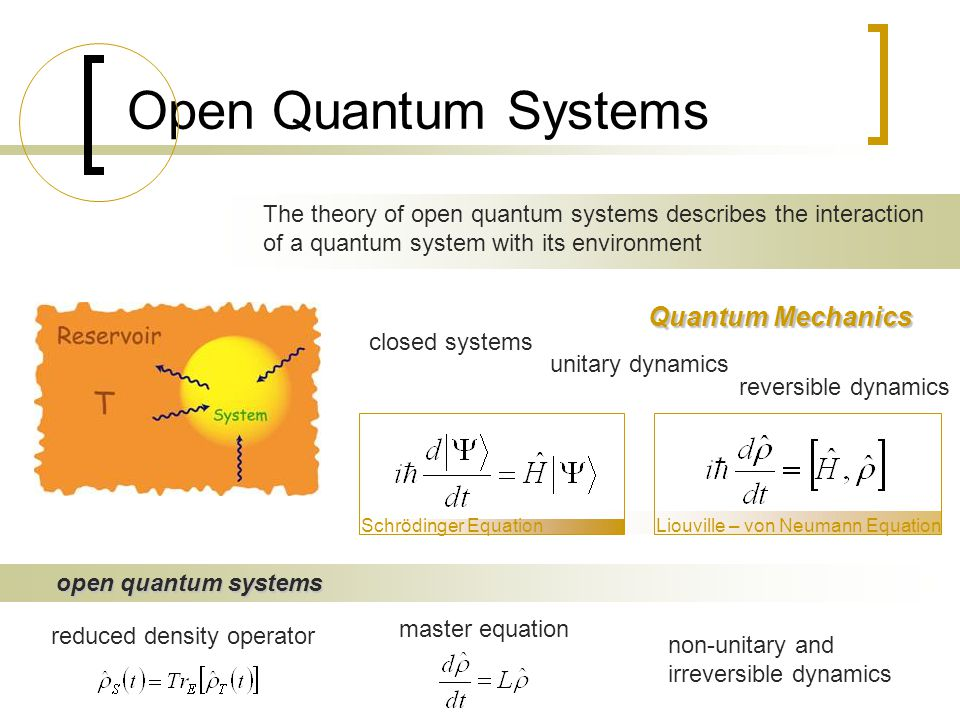
\includegraphics[scale=0.4]{figure/OQS.jpg}
\end{figure}
\end{frame}
%==================================================
\begin{frame}
\frametitle{Non-Hermitian System\footnote{: Zhaoyang Zhang et al 2018 J. Phys. B: At. Mol. Opt. Phys. 51 072001}}

\begin{figure}
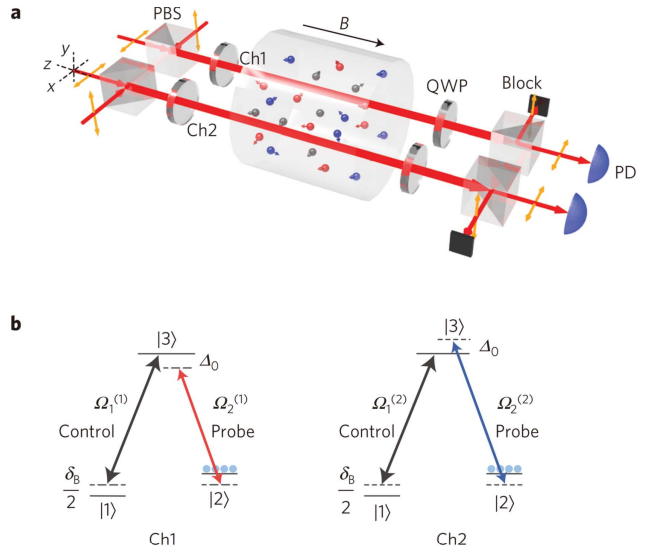
\includegraphics[scale=0.6]{figure/e2.png}
\end{figure}
\end{frame}
%==================================================
\section{SSH Model}
%==================================================
\begin{frame}
\frametitle{SSH Model}
\begin{figure}
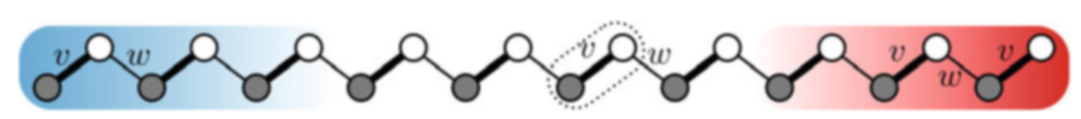
\includegraphics[scale=0.5]{figure/ssh1.png}
\end{figure}
Single-particle Hamiltonian is expressed as
\begin{equation}
H=v\sum_{m=1}^{N}(|m,B\rangle\langle m,A|+h.c)+w\sum_{m=1}^{N-1}(|m+1,A\rangle\langle m,B|+h.c)
\end{equation}
\begin{equation}
H(k)=\mathbf{d}(k)\bf{\hat{\sigma}}
\end{equation}
where $d_x=v+w\cos(k)$, $d_y=w\sin(k)$, $d_z=0$
\begin{equation}
E(k)=\pm\sqrt{v^2+w^2+2vw\cos(k)}
\end{equation}
\end{frame}
%==================================================
\begin{frame}
\frametitle{Winding number}
\begin{figure}
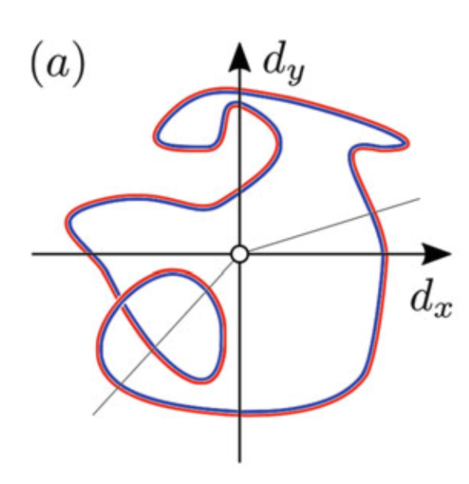
\includegraphics[scale=0.3]{figure/ssh3.png}
\end{figure}
The winding number $v$ is given by
\begin{equation}
v=\frac{1}{2\pi}\int_{-\pi}^{\pi}(\tilde{\mathbf{d}}(k)\times \frac{d}{dk}\tilde{\mathbf{d}}(k))_zdk
\end{equation}
where
$$\tilde{\mathbf{d}}=\frac{\mathbf{d}}{|\mathbf{d}|}$$
\end{frame}
%==================================================
\begin{frame}
\frametitle{Winding number}
\begin{equation}
H(k)=
\left(\begin{array}{cc}
0&h(k)\\
h(k)^*&0
\end{array}\right);\qquad h(k)=d_x(k)-id_y(k)
\end{equation}
Using the complex logarithm function $\log(|h|e^{i\textrm{arg}h})=\log|h|+i\textrm{arg}h$, we have
\begin{equation}
v=\frac{1}{2\pi i}\int_{-\pi}^{\pi}dk\frac{d}{dk}\log h(k)
\end{equation}
\begin{figure}
	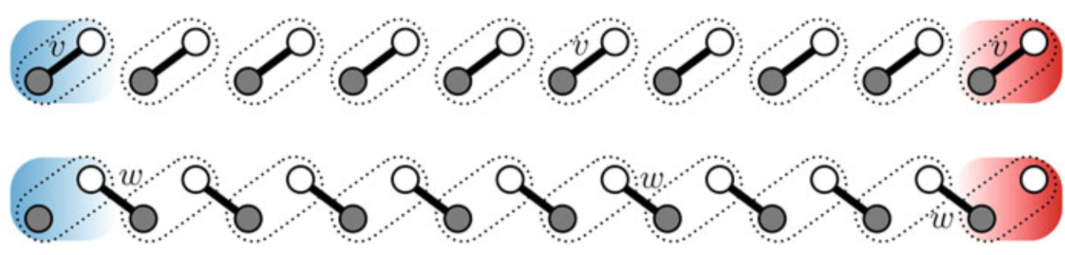
\includegraphics[scale=0.5]{figure/ssh2.png}
\end{figure}
\end{frame}

%==================================================
\section{Non-Hermitian SSH Model}
%======================================================================
  \begin{frame}
    \frametitle{Non-Hermitian SSH Model\footnote{S.Yao,Z.Wang,PRL,121,086803}}
    \begin{figure}
    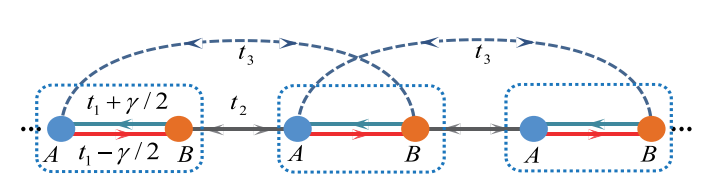
\includegraphics[scale=0.5]{figure/ssh.png}
    \end{figure}
    \begin{equation}
    \begin{aligned}
    H(k)&=d_x\sigma_x+(d_y+i\frac{\gamma}{2})\sigma_y\\
    E(k)&=\sqrt{d_x^2+(d_y+i\frac{\gamma}{2})^2}
    \end{aligned}
   \end{equation}
   
   \begin{equation*}
   d_x=t_1+(t_2+t_3)\cos(k)\qquad d_y=(t_2-t_3)\sin(k)
   \end{equation*}
 Phase transition:\textcolor{red}{$E(k)=0$}
 
Take $t_3=0$, we can derive $(d_x,d_y)=(\pm\gamma/2,0)$ which require $t_1=t_2\pm\frac{\gamma}{2}(k=\pi)$ or $t_1=-t_2\pm\frac{\gamma}{2}(k=0)(\textcolor{red}{\times})$
  \end{frame}
  %====================================================================== 
  \begin{frame}
  \frametitle{Gap close}
  \begin{figure}
  	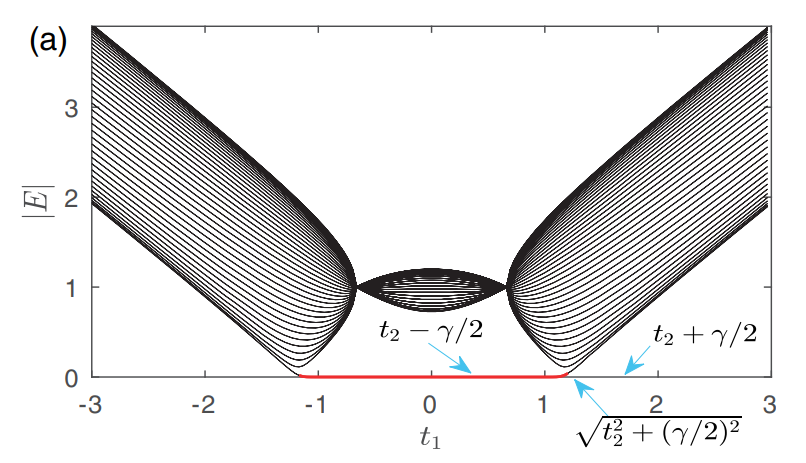
\includegraphics[scale=0.4]{figure/band.png}
  	\caption{Open boundary energy band}
  \end{figure}
\begin{block}{Note}
	\begin{itemize}
	\item\textcolor{red}{ $E(k)=0$ do not correspond phase transition, bulk-boundary correspond is failure.}	
	\end{itemize}
\end{block}
\end{frame}
%==================================================
\begin{frame}
\centering
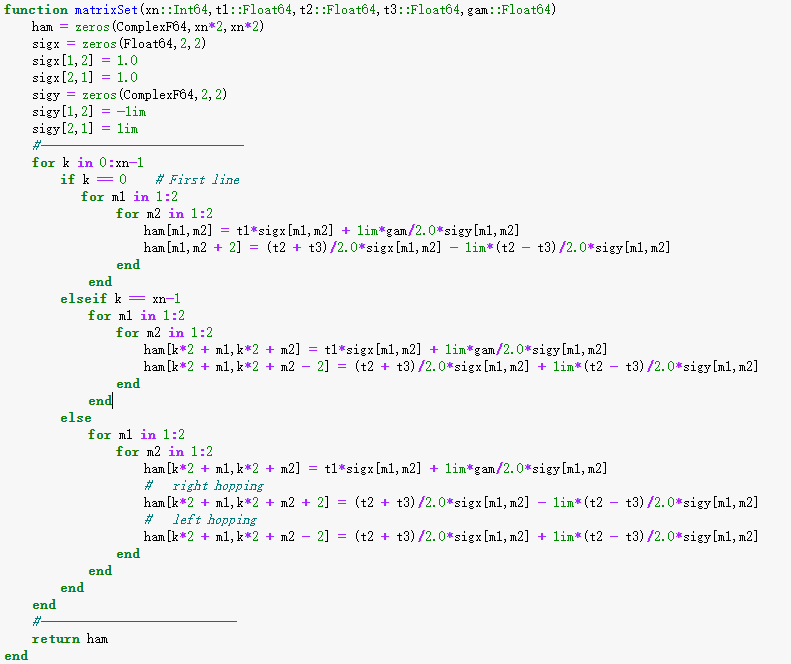
\includegraphics[scale=0.6]{figure/code1.png}
\end{frame}
%=================================================
  \begin{frame}
    \frametitle{Similarity transformation}
    $$\rvert\psi\rangle=(\psi_{1,A},\psi_{1,B},\psi_{2,A},\psi_{2,B},\cdots,\psi_{L,A},\psi_{L,B})^T$$
    \begin{equation}
    H\rvert\psi\rangle=E\rvert\psi\rangle\Leftrightarrow	\bar{H}\rvert\bar{\psi}\rangle=E\rvert\bar{\psi}\rangle\quad \text{with}\quad \rvert\bar{\psi}\rangle=S^{-1}\rvert\psi\rangle
    \end{equation}
    \begin{equation}
    \textcolor{red}{\bar{H}=S^{-1}HS}
    \end{equation}
    $$S=\{1,r,r,r^2,r^2,\cdots,r^{L-1},r^{L-1},r^L\}$$
    For $\bar{H}:$ $t_1\pm\frac{\gamma}{2}\rightarrow r^{\pm 1}(t_1+\pm\frac{\gamma}{2})$, if take \textcolor{blue}{$r=\sqrt{|(t_1-\gamma/2)/(t_1+\gamma/2)|}$}, $\bar{H}$ becomes the standard SSH model for $|t_1|>|\gamma/2|$, with intracell and intercell hoppings 
    \begin{equation}
    \bar{t}_1=\sqrt{(t_1-\gamma/2)(t_1+\gamma/2)},\quad \bar{t}_2=t_2
    \end{equation}
   
  \end{frame}

  %====================================================================== 
  \begin{frame}
  \frametitle{Gap close}
  \begin{equation}
  \bar{H}(k)=(\bar{t}_1+\bar{t}_2\cos(k))\sigma_x+\bar{t}_2\sin(k)\sigma_y
  \end{equation}
  Phase transition: \textcolor{red}{$E(k)=0$} $\rightarrow \bar{t}_1=\bar{t}_2$
  \begin{equation}
  t_1=\pm\sqrt{t_2^2+(\gamma/2)^2}\qquad(\textcolor{red}{\checkmark})
  \end{equation} 
  \begin{block}{Note}
  With the help of similarity transformation, Non-Hermitian SSH model can be modified to Hermitian SSH model, energy gap closure could perdict phase transition.
  \end{block}
  \end{frame}

  %======================================================================
  \begin{frame}
    \frametitle{Generalizable solution}
    Real space eigen-equation is 
    \begin{equation}
    \begin{aligned}
    t_2\psi_{n-1,B}+\left[t_1+(\gamma/2)\right]\psi_{n,B}=&sE\psi_{n,A}\\
    \left[t_1-(\gamma/2)\right]\psi_{n,A}+t_2\psi_{n+1,A}=&E\psi_{n,B}
    \end{aligned}
    \end{equation}
    Take the ansatz that $|\psi\rangle=\sum_j|\phi^{(j)}\rangle$, where each $|\phi^{(j)}\rangle$ takes the exponential form: $(\phi_{n,A},\phi_{n,B})=\beta^n(\phi_A,\phi_B)$, which satisfies
    \begin{equation}
    \begin{aligned}
    \left[t_1+\frac{\gamma}{2}+t_2\beta^{-1}\right]\phi_B=&E\phi_A\\
    \left[(t_1-\frac{\gamma}{2})+t_2\beta\right]\phi_A=&E\phi_B
    \end{aligned}
    \end{equation}
    Therefore, we have
    \begin{equation}
    \left[(t_1-\frac{\gamma}{2})+t_2\beta\right]\left[(t_1+\frac{\gamma}{2})+t_2\beta^{-1}\right]=E^2\label{2ndeq}
    \end{equation}
  \end{frame}
  %====================================================================== 
  \begin{frame}
  \frametitle{Generalizable solution}
  two solutions
  \begin{scriptsize}
 \begin{equation}
 \beta_{1,2}(E)=\left[E^2+\gamma^2/4-t_1^2+t_2^2\pm\sqrt{(E^2+\gamma^2/4-t_1^2-t_2^2)^2-4t_2^2(t_1^2-\gamma^2/4)}\right]/\left[2t_2(t_1+\gamma/2)\right]
 \end{equation}
  \end{scriptsize}
  In the $E\rightarrow 0$ limit, we have
  \begin{equation}
  \beta_{1,2}^{E\rightarrow 0}=-\frac{t_1-\gamma/2}{t_2},\quad -\frac{t_2}{t_1+\gamma/2}
  \end{equation}
  These two solutions correspond to $\phi_B=0$ and $\phi_A=0$, respectively.
  
  Restoring the $j$ index $|\phi^{(j)}\rangle$, we have
  \begin{equation}
  \phi_A^{(j)}=\frac{E}{t_1-\gamma/2+t_2\beta}\phi_B^{(j)},\quad \phi_B^{(j)}=\frac{E}{t_1+\gamma/2+t_2\beta^{-1}}\phi_A^{(j)}\label{jd}
  \end{equation}
\end{frame}
  
  %============================================================
    \begin{frame}
  \frametitle{Generalizable solution}
  The general solution is writted as a linear combination
  \begin{equation}
  \left(\begin{array}{c}
  \Psi_{n,A} \\ 
  \Psi_{n,B}
  \end{array} \right)=\beta_1^n\left(\begin{array}{c}
  \phi_{A}^{(1)} \\ 
  \phi_{B}^{(1)}
  \end{array}\right)+\beta_2^n\left(\begin{array}{c}
  \phi_{A}^{(2)} \\ 
  \phi_{B}^{(2)}
  \end{array}\right)
  \end{equation}
  Boundary condition
  \begin{equation}
  \begin{aligned}
  (t_1+\gamma/2)\Psi_{1,B}-E\Psi_{1,A}=&0\\
  (t_1-\gamma/2)\Psi_{L,A}-E\Psi_{L,B}=&0
  \end{aligned}
  \end{equation}
  Together with (\ref{jd}), they lead
  \begin{equation}
  \beta_1^{L+1}(t_1-\gamma/2+t_2\beta_2)=\beta_2^{L+1}(t_1-\gamma/2+t_2\beta_1)
  \end{equation}
  We are concerned about the spectrum for a long chain, which necessitates \textcolor{red}{$|\beta_1|=|\beta_2|$} for the bulk eigenstates.
\end{frame}
  
  %==========================================================
  \begin{frame}
  \frametitle{Generalizable solution}
  Combined with $\beta_1\beta_2=(t_1-\gamma/2)/(t_1+\gamma/2)$, $|\beta_1|=|\beta_2|$ leads to 
  \begin{equation}
  |\beta_j|=r\equiv\sqrt{\rvert\frac{t_1-\gamma/2}{t_1+\gamma/2}\rvert}\label{gbz}
  \end{equation}
  \begin{figure}
  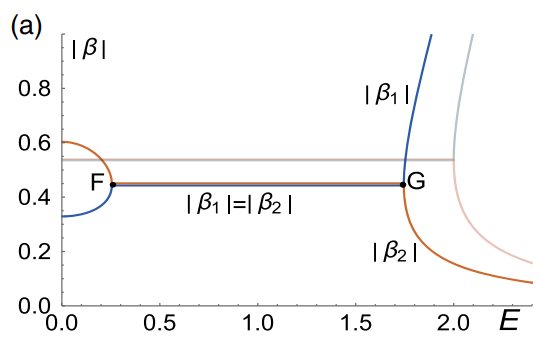
\includegraphics[scale=0.5]{figure/beta.png}
  \caption{The excepted $|\beta_1|=|\beta_2|=r$ relation is found on the line FG, which is associated with bulk spectra.}
  \end{figure}
\end{frame}

%==========================================================
\begin{frame}
\frametitle{Generalizable solution}
Take $\beta=re^{ik}(k\in\left[0,2\pi\right])$ into (\ref{2ndeq}) to obtain the spectra
\begin{scriptsize}
\begin{equation}
E^2(k)=t_1^2+t_2^2-\gamma^2/4+t_2^2\sqrt{|t_1^2-\gamma^2/4|}\left[\text{sgn}(t_1+\gamma/2)e^{ik}+\text{sgn}(t_1-\gamma/2)e^{-ik}\right]
\end{equation}
\end{scriptsize}
whihc recovers the spectrum of SSH model when $\gamma=0$. The phase transition points can be predicted when $|E(k)|=0$
\begin{figure}[f]
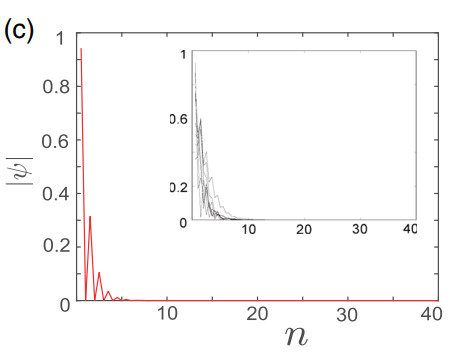
\includegraphics[scale=0.5]{figure/NSEF.png}
\end{figure}
The usual Bloch wave carry a pure phase factor $e^{ik}$, whose role is now played by $\beta$. In addition to the phase factor, $\beta$ has a modulus $|\beta|\neq 1$ in general.
\end{frame}
  
  %============================================================
  \section{Non-Bloch invariant}

  %======================================================================
  \begin{frame}
    \frametitle{Winding Number}
    We start from the non-Bloch Hamiltonian obtained from $H(k)$ by the replacement $e^{ik}\rightarrow \beta$, $e^{-ik}\rightarrow \beta^{-1}$:
    \begin{equation}
    H(\beta)=(t_1-\frac{\gamma}{2}+\beta t_2)\sigma_{-}+(t_1+\frac{\gamma}{2}+\beta^{-1}t_2)\sigma_{+}
    \end{equation}
    where $\sigma+{\pm}=(\sigma_x\pm i\sigma_y)/2$, $\beta$ takes values in a nonunit circle $|\beta|=r$(in other words,$k$ acquires an imaginary part $-i\ln r$)
    \begin{figure}
    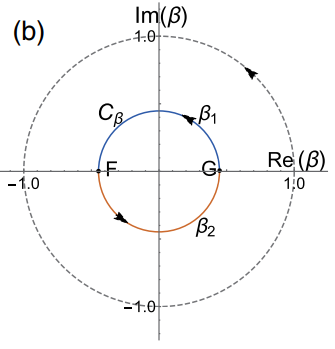
\includegraphics[scale=0.5]{figure/gbz.png}
    \end{figure}
    
  \end{frame}
  %======================================================================

  %======================================================================
  \begin{frame}
    \frametitle{Winding Number}
    \begin{equation}
    H(\beta)|u_R\rangle=E(\beta)|u_R\rangle,\quad H^\dagger(\beta)|u_L\rangle=E^{*}(\beta)|u_L\rangle
    \end{equation}
    Chiral symmetry ensures that $|\tilde{u}_R\rangle\equiv\sigma_z|u_R\rangle$ and $|\tilde{u}_L\rangle\equiv\sigma_z|u_L\rangle$.  $H(\beta)=TJT^{-1}$ with $J=\left(\begin{array}{cc}
    E&0\\
    0&-E
    \end{array}\right)$, and the normalization condition $\langle u_L|u_R\rangle=\langle\tilde{u}_L|\tilde{u}_R\rangle=1$, $\langle u_L|\tilde{u}_R\rangle=\langle \tilde{u}_L|u_R\rangle=0$
    
    Q matrix can be expressed as:
    \begin{equation}
    Q(\beta)=|\tilde{u}_R(\beta)\rangle\langle \tilde{u}_L(\beta)|-|u_R(\beta)\rangle\langle u_L(\beta)|
    \end{equation}
    which is off-diagonal due to chiral symmetry $\sigma_z^{-1}Q\sigma_z=-Q$, namely, $Q=\left(\begin{array}{cc}
    0&q\\
    q^{-1}&0
    \end{array}\right)$
  \end{frame}
%==================================================
\begin{frame}
\begin{figure}
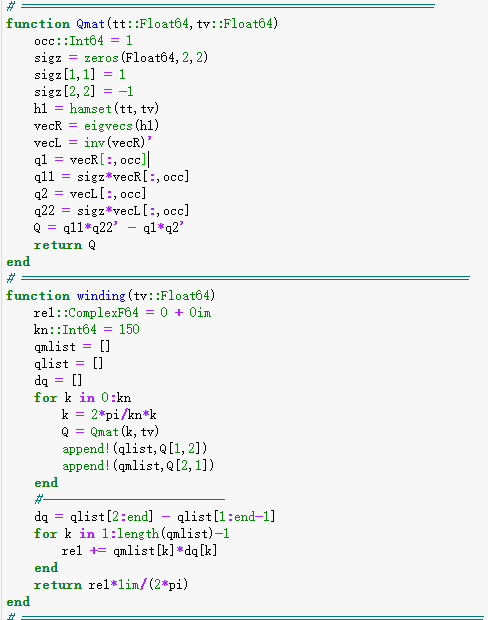
\includegraphics[scale=0.65]{figure/code2.png}
\end{figure}
\end{frame}
%==================================================
   \begin{frame}
  \frametitle{Winding Number}
  Non-Bloch winding number:
  \begin{equation}
  W=\frac{i}{2\pi}\int_{C_\beta}q^{-1}dq
  \end{equation}
  \begin{figure}
  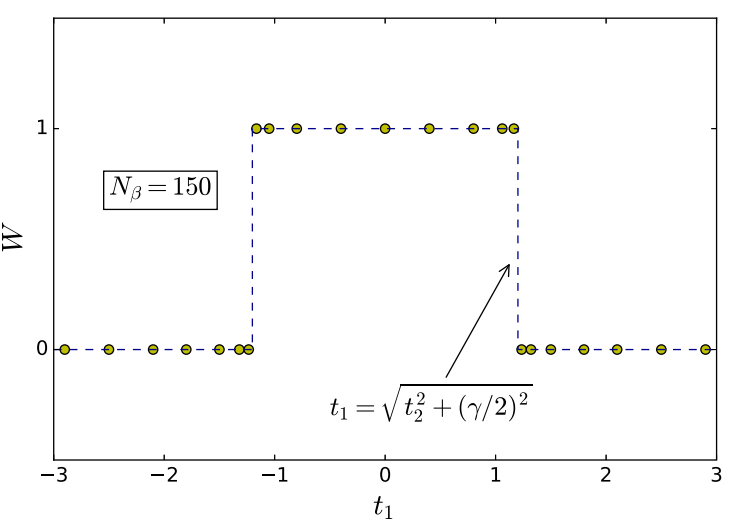
\includegraphics[scale=0.28]{figure/wind.png}
  \end{figure}

  
\begin{block}{Note}
Crucially, it is defined on the "generalized Brillouin zone" $C_{\beta}$. The image of high-dimensional GBZ is not very clear. 
\end{block}
\end{frame}
%==================================================
\section{Non-Bloch Chern Band}
%==================================================
\begin{frame}
\frametitle{Non-Hermitian Chern insulator\footnote{S.Yao,F.Song,Z.Wang,PRL,121,136802}}
\begin{footnotesize}
\begin{equation}
H(\mathbf{k})=(v_x\sin(k_x)+i\gamma_x)\sigma_x+(v_y\sin(k_y)+i\gamma_y)\sigma_y+(m-t_x\cos(k_x)-t_y\cos(k_y)+i\gamma_z)\sigma_z
\end{equation}
\end{footnotesize}

\begin{footnotesize}
\begin{equation}
E_{\pm}(\mathbf{k})=\pm\sqrt{\sum_{j=x,y,z}(h_j^2-\gamma_j^2+2i\gamma_jh_j)}
\end{equation}
\end{footnotesize}
where $(h_x,h_y,h_z)=(v_x\sin(k_x),v_y\sin(k_y),v_z\sin(k_z))$.

The Bloch bands are gapped if $$E_{\pm}(\mathbf{k})\neq 0\Rightarrow m>m_+\quad \textrm{and}\quad m<m_{-}$$

For $\gamma_z=0$
\begin{equation}
m_{\pm}=t_x+t_y\pm\sqrt{\gamma_x^2+\gamma_y^2}
\end{equation}
\textcolor{blue}{$H(\mathbf{k})$-based Chern number is nondefinable in the gapless region $m\in\left[m_{-},m_{+}\right]$}
\end{frame}
%==================================================
\begin{frame}
\frametitle{Topological phase diagram}
\begin{figure}
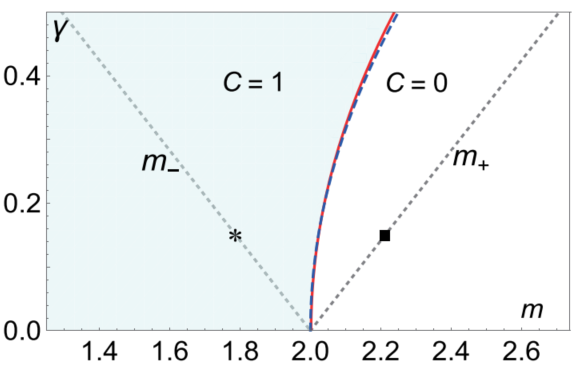
\includegraphics[scale=0.3]{figure/2d-1.png}
\end{figure}
\begin{figure}
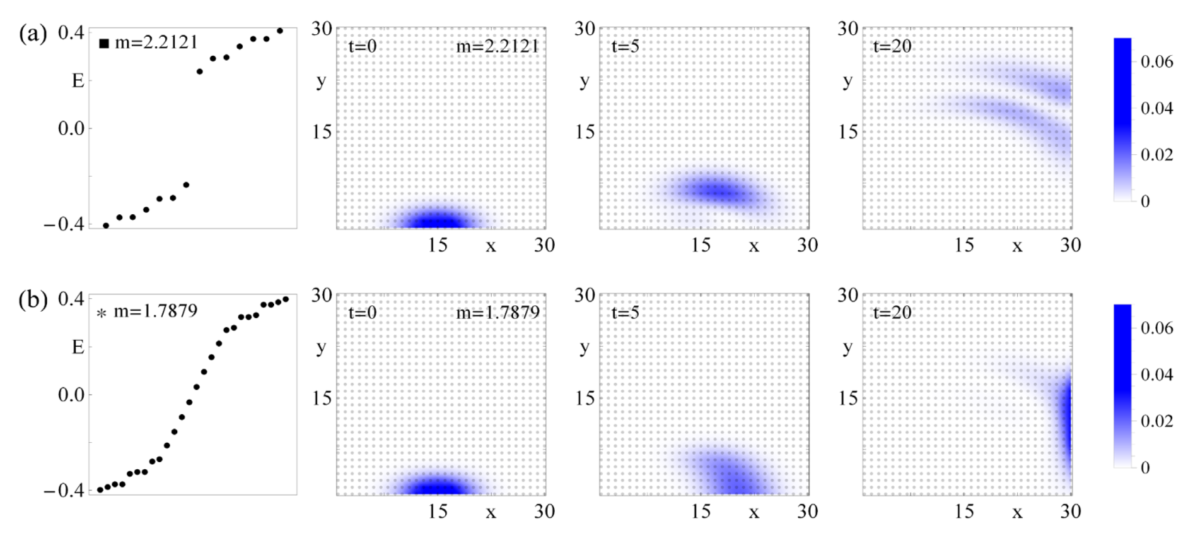
\includegraphics[scale=0.4]{figure/2d-2.png}
\end{figure}
\end{frame}
%==================================================
\begin{frame}
\frametitle{Non-Bloch Chern number}
To describe open-boundary eigenstates
$$\mathbf{k}\rightarrow \tilde{\mathbf{k}}+i\tilde{\mathbf{k}}'$$
Define a "non-Bloch Hamiltonian" as follows:
$$\tilde{H}(\tilde{\mathbf{k}})\equiv H(\mathbf{k}\rightarrow \tilde{\mathbf{k}}+i\tilde{\mathbf{k}}')$$
$\tilde{H}(\tilde{\mathbf{k}})$ is generally non-Hermitian, we define the standard right or left eigenvector by
\begin{equation}
\tilde{H}(\tilde{\mathbf{k}})|u_{R\alpha}\rangle=E_{\alpha}|u_{R\alpha}\rangle\quad \tilde{H}(\tilde{\mathbf{k}})^\dagger|u_{L\alpha}\rangle=E^*_\alpha|u_{L\alpha}\rangle
\end{equation}
The normalization $\langle u_{L\alpha}|u_{R\alpha}\rangle=1$ is required in defining Chern numbers.
\end{frame}
%==================================================
\begin{frame}
\frametitle{Non-Bloch Chern number}
\begin{equation}
C_\alpha=\frac{1}{2\pi i}\int_{\tilde{T}^2}d^2\mathbf{\tilde{k}}\epsilon^{ij}\langle \partial_iu_{L\alpha}(\tilde{\mathbf{k}})|\partial_ju_{R\alpha}(\tilde{\mathbf{k}})\rangle
\end{equation}
Focus on the Chern number of "valence band"Re($E_ \alpha<0$), compute the Chern number from $\tilde{H}(\tilde{\mathbf{k}})$, when $t_{x,y}=v_{x,y}=1$, $\gamma_{x,y}=\gamma$, the phase boundary is 
\begin{equation}
m=2+\gamma^2
\end{equation}
\begin{figure}
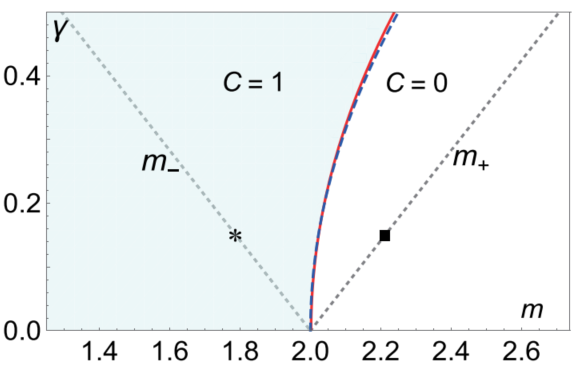
\includegraphics[scale=0.45]{figure/2d-1.png}
\end{figure}
\end{frame}
%==================================================
\section{Progress}
%=================================
\begin{frame}
\frametitle{Non-Hermitian Research}
\begin{itemize}
	\item Higher-order non-Hermitian skin effect\\
	(PRB,102,205118)
	\item Non-Hermitian nodal-line semimetal\\
	(PRB,99,075130)
	\item \textcolor{red}{DMFT Reveals the Non-Hermitian Topology and Fermi Arcs in Heavy-Fermion Systems}\\
	(PRL,125,227204)
	\item Parity-time-symmetric topological superconductor\\
	(PRB,98,085116)
	\item Defective Majorana zero modes in non-Hermitian Kitaev chain\\
	(Arxiv,2010,11451)
	\item \dots
\end{itemize}
\end{frame}

\end{document} 